\documentclass[specialist,
substylefile = spbu_report.rtx,
subf,href,colorlinks=true, 12pt]{disser}

\usepackage[a4paper,
mag=1000, includefoot,
left=1.5cm, right=1.5cm, top=2cm, bottom=2cm, headsep=1cm, footskip=1cm]{geometry}

\usepackage{color}
\definecolor{black}{RGB}{0,0,0}

%\usepackage{hyperref}
\usepackage{mathtext}
\usepackage{outlines}
\usepackage{amsmath,amssymb,amsthm,amscd,amsfonts}
\usepackage{cmap}
\usepackage[utf8]{inputenc}
\usepackage[T2A]{fontenc}
\usepackage[russian]{babel}
\usepackage{euscript}
\usepackage{mathdots}
\usepackage{graphicx}
%\usepackage[colorlinks,citecolor=black, linkcolor=black]{hyperref}
\usepackage[russian]{cleveref}
\usepackage{epstopdf}
\usepackage{longtable} 
\usepackage{multirow}
\usepackage{float}
\usepackage{wrapfig}
\usepackage{caption}
\usepackage{esdiff}
\usepackage{mathtools, bigstrut}
\usepackage[shortlabels]{enumitem}
\usepackage{listings}
\usepackage{setspace}
\usepackage{xcolor}
\usepackage{minted}
\usepackage{epstopdf}
\usepackage{array}


\newtheorem*{theorem}{Теорема}
\newtheorem*{Corollary}{Следствие}
\newtheorem*{Remark}{Замечание}
\newtheorem*{Lemma}{Лемма}
\newtheorem*{Definition}{Определение}
\newcommand*\rfrac[2]{{}^{#1}\!/_{#2}}
%\newcommand{\tg}[1]{\mathrm{tg} \left(#1\right)}
\sectionfont{\fontsize{18}{15}\selectfont}
\subsectionfont{\fontsize{16}{13}\selectfont}
\subsubsectionfont{\fontsize{14}{11}\selectfont}
%\DeclareMathOperator{\deter}{det}
\DeclareMathOperator{\rk}{rk}
\DeclareMathOperator{\re}{Re}
\DeclareMathOperator{\im}{Im}
%\DeclareMathOperator{\arctg}{arctg}


\definecolor{codegreen}{rgb}{0,0.6,0}
\definecolor{codegray}{rgb}{0.5,0.5,0.5}
\definecolor{codepurple}{rgb}{0.58,0,0.82}
\definecolor{backcolour}{rgb}{0.95,0.95,0.92}

%Code listing style named "mystyle"
\lstdefinestyle{mystyle}{
	backgroundcolor=\color{backcolour}, commentstyle=\color{codegreen},
	keywordstyle=\color{red},
	numberstyle=\tiny\color{codegray},
	stringstyle=\color{blue},
	basicstyle=\ttfamily\footnotesize,
	breakatwhitespace=false,         
	breaklines=true,                 
	captionpos=b,                    
	keepspaces=true,                 
	numbers=left,                    
	numbersep=5pt,                  
	showspaces=false,                
	showstringspaces=false,
	showtabs=false,                  
	tabsize=2
}

%"mystyle" code listing set
\lstset{style=mystyle}


\AtBeginDocument{\addtocontents{toc}{\protect\thispagestyle{plain}}} 
\setcounter{tocdepth}{2}
%\linespread{1} 
\begin{document}
	
	%
	% Титульный лист на русском языке
	%
	% Название организации
	\institution{%		
		\begin{spacing}{1}
			Министерство науки и высшего образования Российской Федерации\\
			\textbf{--------------------------------}\\
			Санкт-Петербургский политехнический университет Петра Великого\\
			Высшая школа программной инженерии
		\end{spacing}
	}
	
	\title{\textbf{КУРСОВАЯ РАБОТА}}
	
	% Тема
	\topic{по дисциплине «Базы данных»\\		
		\textbf{\\Графический интерфейс пользователя для базы данных «Госпиталь»}}
	
	% Автор
	\author{Зайцев В.А.}
	\group{студент гр. 5130904/30103}
	
	% Научный руководитель
	\sa       {Прокофьев О.В.}
	%\sastatus {проф, д.т.н. }
	
	% Город и год
	\city{Санкт-Петербург}
	\date{\number\year}
	
	\maketitle
	\pagestyle{plain}
	\newpage
	\tableofcontents
	
	\section{Задание}
	Целью данной курсовой работы является создание приложения, включающего в себя клиентскую часть GUI для Базы Данных «Госпиталь». Приложение должно включать в себя следующие элементы:
	\vspace{-5pt}
	\begin{itemize}
		\setlength{\itemsep}{-2pt}
		\item[а)] отдельный файл параметров подключения к БД, который задаются файлом (формат plain text file или ini config file или xml file);
		\item[б)] авторизацию с хешированием паролей для пользователей (2 пользователя);
		\item[в)] меню приложения содержит группы элементов: СПРАВОЧНИКИ, ЖУРНАЛЫ, ОТЧЕТЫ;
		\item[г)] приложение должно обеспечивать ввод, редактирование, просмотр информации из БД;
		\item[д)] используется пользовательский элементы вида GridView для обзора таблиц (представлений) БД;
		\item[е)] GridView, который содержит внешние ключи, должен содержать нужные/необходимые атрибуты внешней таблицы.
		\item[ж)] есть отдельная форма для работы с записью таблицы, содержащая эл-ты интерфейса ДОБАВИТЬ, ИЗМЕНИТЬ, УДАЛИТЬ, ЗАКРЫТЬ; открывается из GridView
		\item[з)] меню пункта ОТЧЕТЫ вызывает формы вывода отчетов (минимум 2-х) (выходной формат txt или xls или pdf).
	\end{itemize}
	
	\newpage
	\section{Пользователи базы данных}
	Для работы с БД было создано 2 основных роли пользователя, пароли которых захешированы с помощью модифицированного алгоритма Blowfish:
	\begin{enumerate}
		\item basic\_role – наделена правами чтения, вставки, удаления и изменения для таблицы Пациенты, а также правами на чтение для таблиц Палаты и Диагнозы.
		\item advanced\_role – наделена правами чтения, вставки, удаления и изменения для таблиц Пациенты, Палаты и Диагнозы.
	\end{enumerate}

	Для хранения записей о пользователях была создана таблица users с полями id, username и password\_hash:
	\begin{table}[h]
		\centering
		\renewcommand{\arraystretch}{1.5}
		\begin{tabular}{|c|c|c|}
			\hline
			\textbf{id} & \textbf{username} & \textbf{passord\_hash} \\
			\hline
			1 & basic\_user &\$2b\$12\$tmkj48MYoZNnAZbsQ4tc1uyZLY/xwdwNgQq9G5JnlU900XWeSIe6G \\
			\hline
			2 & advanced\_user &\$2b\$12\$oIXeR7OnlssIOBuOh9X1kuRGZuuafwE8nTA7jAJwpPp7Eoja4nfG. \\
			\hline
		\end{tabular}
	\end{table}
	
	\noindent В ней хранятся имя пользователя и хеш пароля, который формируется с индивидуальной солью. Для подключения используются параметры заданные в ini файле config.ini:
	\vspace{-5pt}
	\inputminted[
	bgcolor=gray!5,
	frame=single,
	style=vs
	]{ini}{../config.ini}
	\indent По умолчанию пользователь app\_user имеет роль waitroom\_role, которая имеет права только на чтение таблицы пользователей, и при успешной авторизации пользователю устанавливается роль basic\_role или advanced\_role.
	
	\section{Работа интерфейса}
	\subsection{Вход}
	\begin{figure}[H]
		\centering
		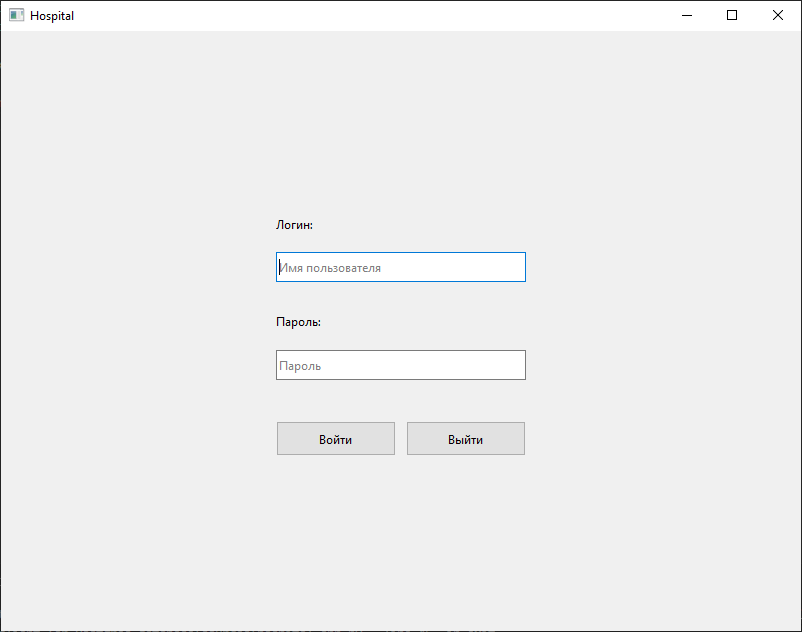
\includegraphics[width=\textwidth]{images/log_window_0.png}
		\caption[]{Окно входа}
	\end{figure}
	\begin{figure}[H]
		\centering
		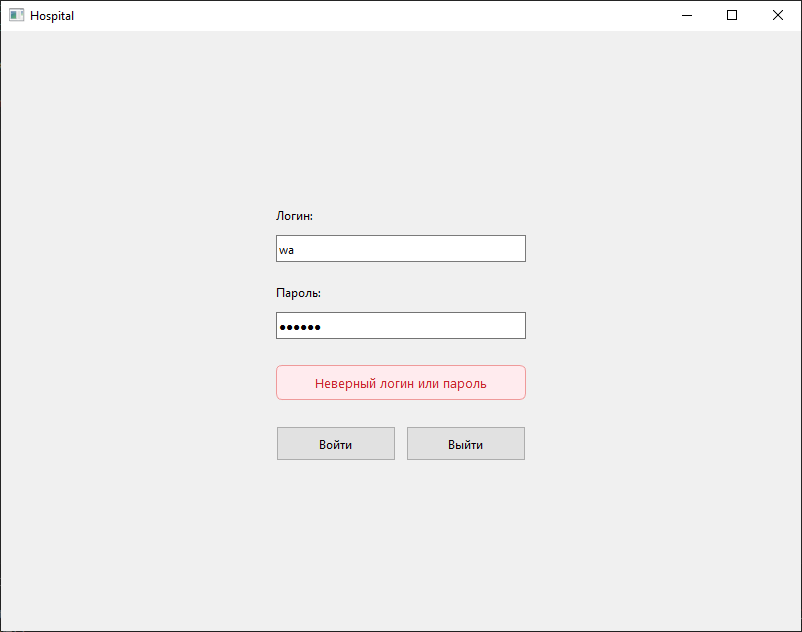
\includegraphics[width=\textwidth]{images/log_window_1.png}
		\caption[]{Неверный логин или пароль}
	\end{figure}
	\begin{figure}[H]
		\centering
		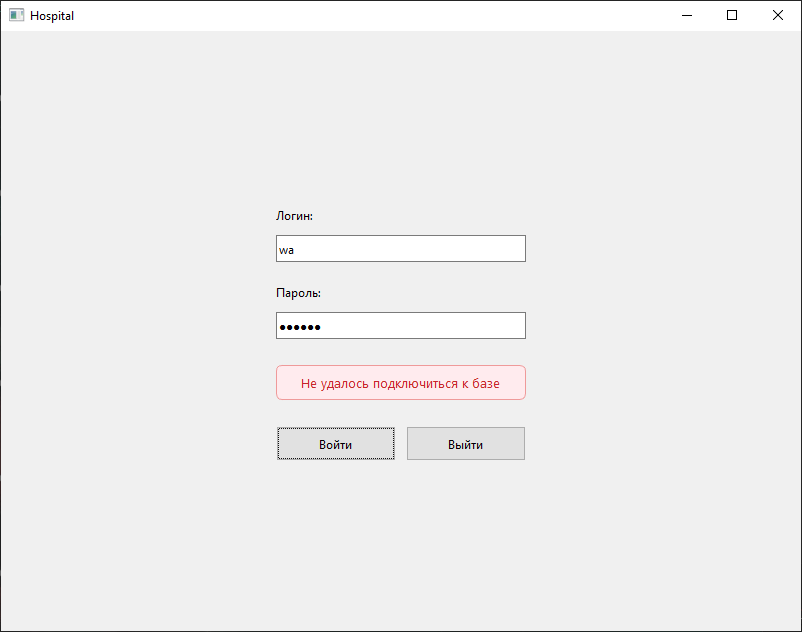
\includegraphics[width=\textwidth]{images/log_window_2.png}
		\caption[]{Отсутствие подключения к базе}
	\end{figure}
	\subsection{Основной интерфейс}
	\subsubsection{Журналы}
		\begin{figure}[H]
			\centering
			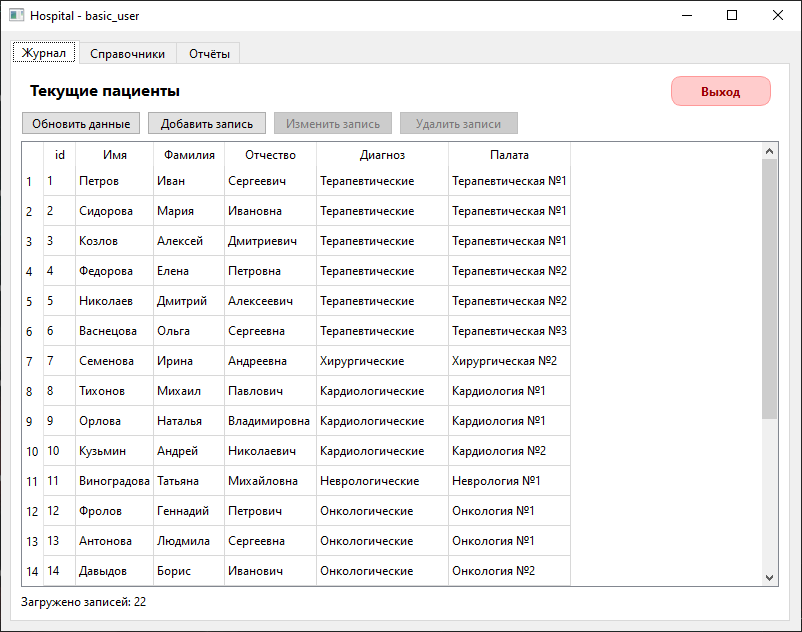
\includegraphics[width=\textwidth]{images/main_widget_0.png}
			\caption[]{Таблица пациентов}
		\end{figure}
		\begin{figure}[H]
			\centering
			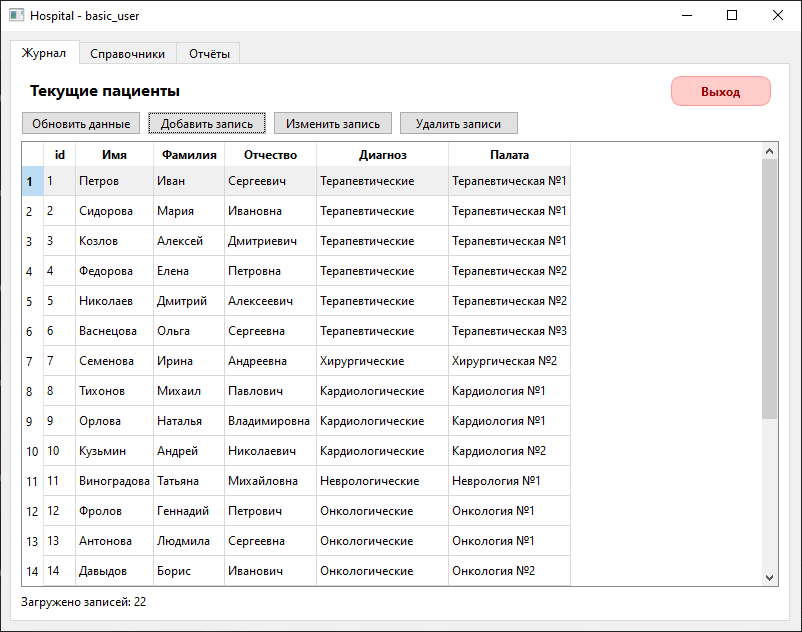
\includegraphics[width=\textwidth]{images/main_widget_1.png}
			\caption[]{Изменение состояний кнопок при выборе записей}
		\end{figure}
		\begin{figure}[H]
			\centering
			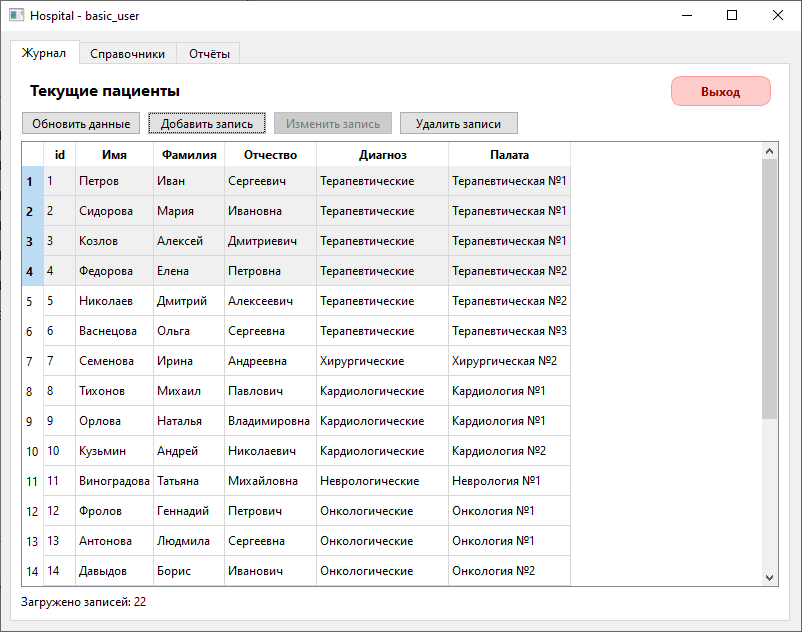
\includegraphics[width=\textwidth]{images/main_widget_2.png}
			\caption[]{Изменение состояний кнопок при выборе записей}
		\end{figure}
				\begin{figure}[H]
			\centering
			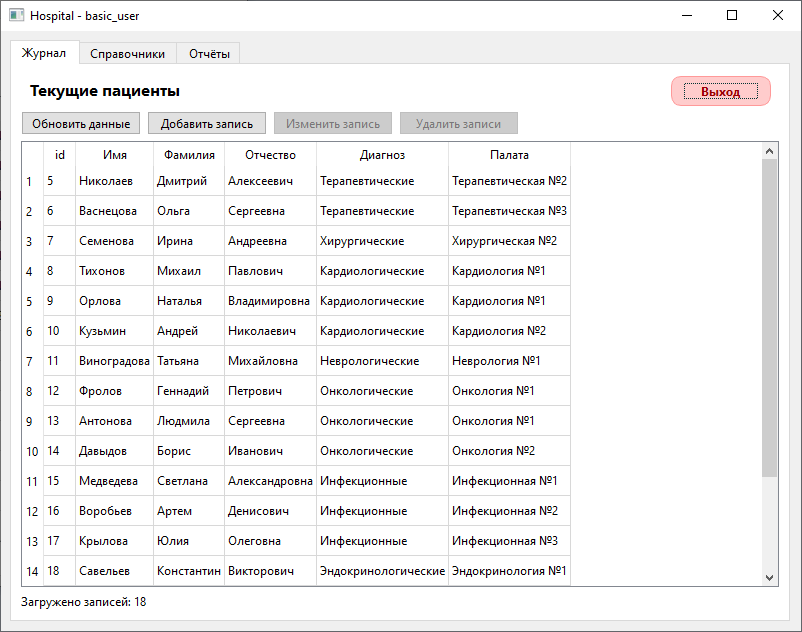
\includegraphics[width=\textwidth]{images/main_widget_3.png}
			\caption[]{Результат удаления}
		\end{figure}
		\begin{figure}[H]
			\centering
			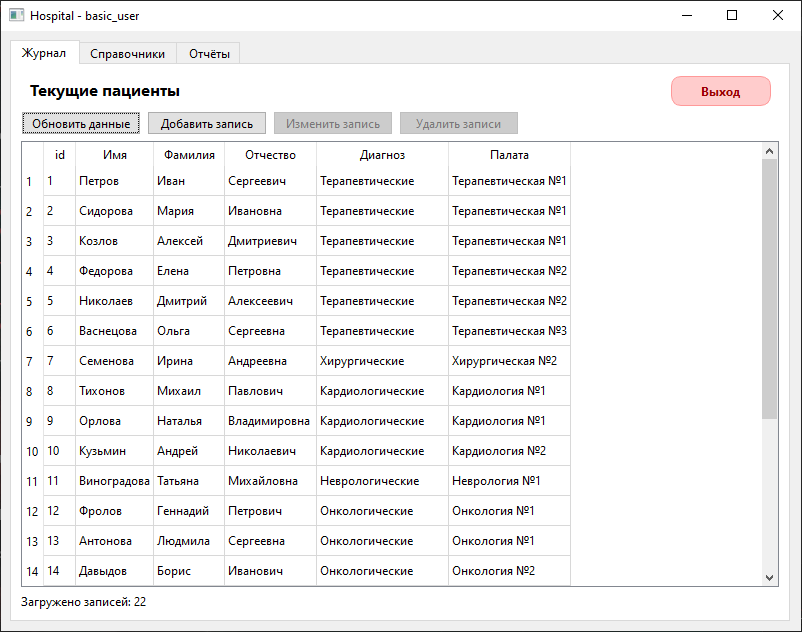
\includegraphics[width=\textwidth]{images/main_widget_4.png}
			\caption[]{Неверный логин или пароль}
		\end{figure}
		\begin{figure}[H]
			\centering
			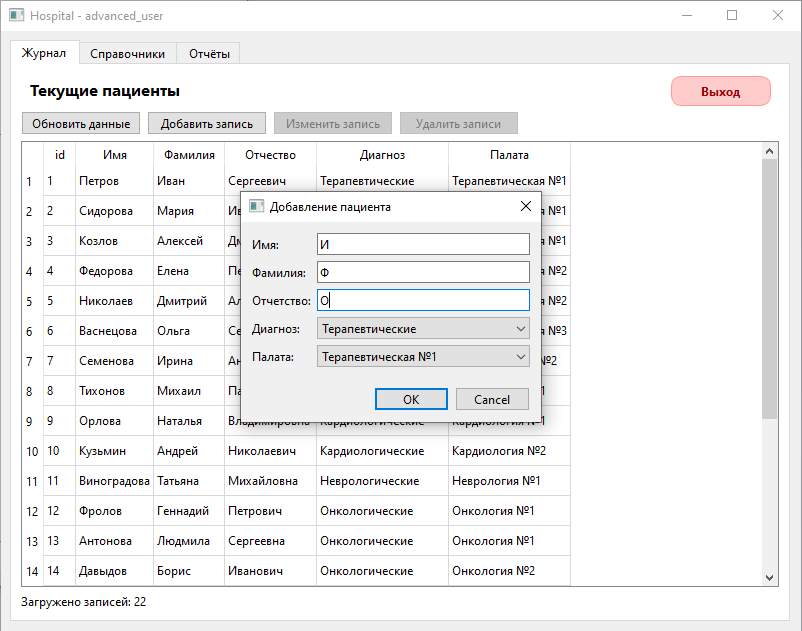
\includegraphics[width=\textwidth]{images/main_widget_5.png}
			\caption[]{Окно добавления пациента}
		\end{figure}
				\begin{figure}[H]
			\centering
			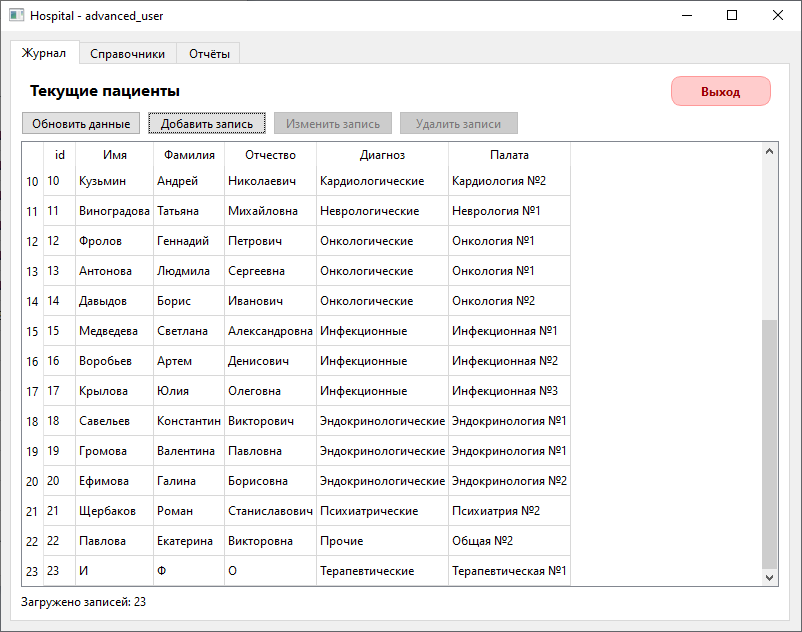
\includegraphics[width=0.75\textwidth]{images/main_widget_6.png}
			\caption[]{Результат добавления пациента}
		\end{figure}
		\begin{figure}[H]
			\centering
			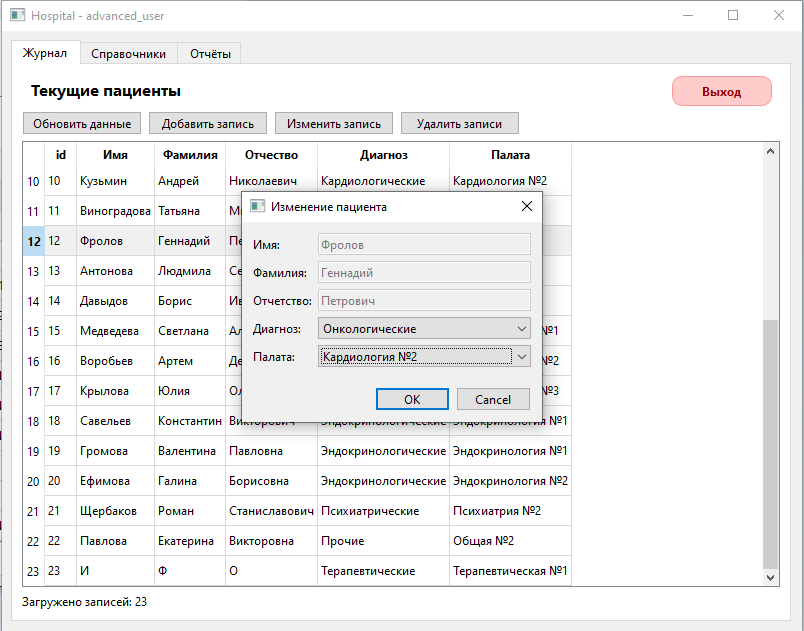
\includegraphics[width=0.75\textwidth]{images/main_widget_7.png}
			\caption[]{Окно изменения пациента}
		\end{figure}
		\begin{figure}[H]
			\centering
			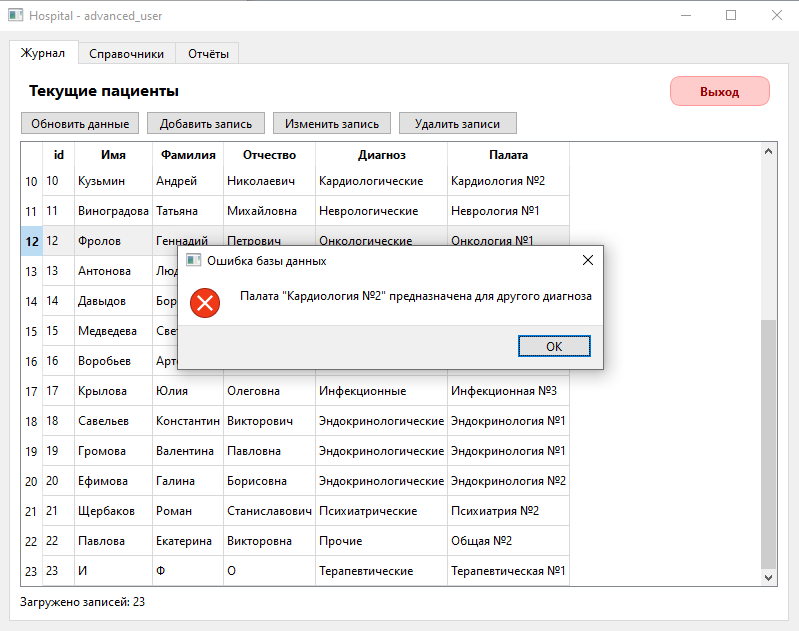
\includegraphics[width=0.75\textwidth]{images/main_widget_8.png}
			\caption[]{Ошибки при выборе некорректных данных}
		\end{figure}
		
	\subsubsection{Справочники}
		\begin{figure}[H]
			\centering
			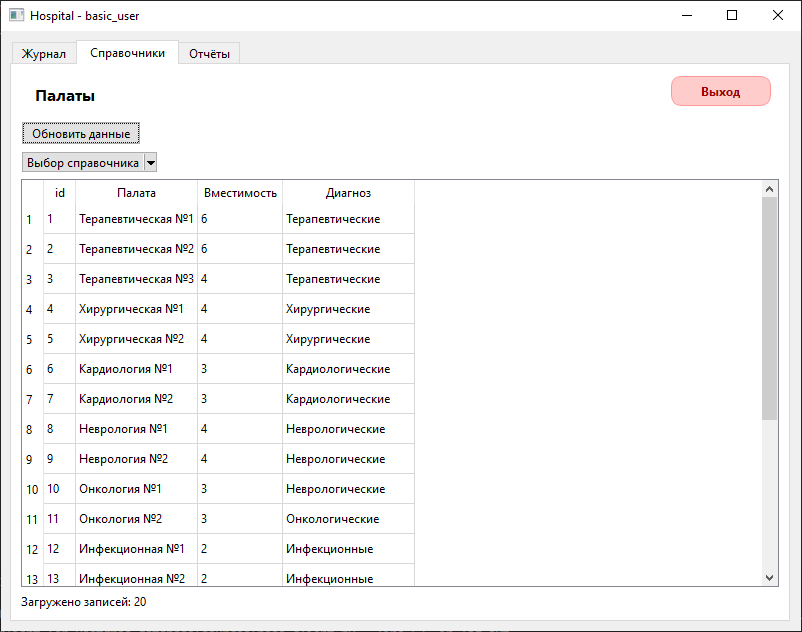
\includegraphics[width=0.75\textwidth]{images/directories_widget_0.png}
			\caption[]{Таблица палат для пользователя basic\_user}
		\end{figure}
		\begin{figure}[H]
			\centering
			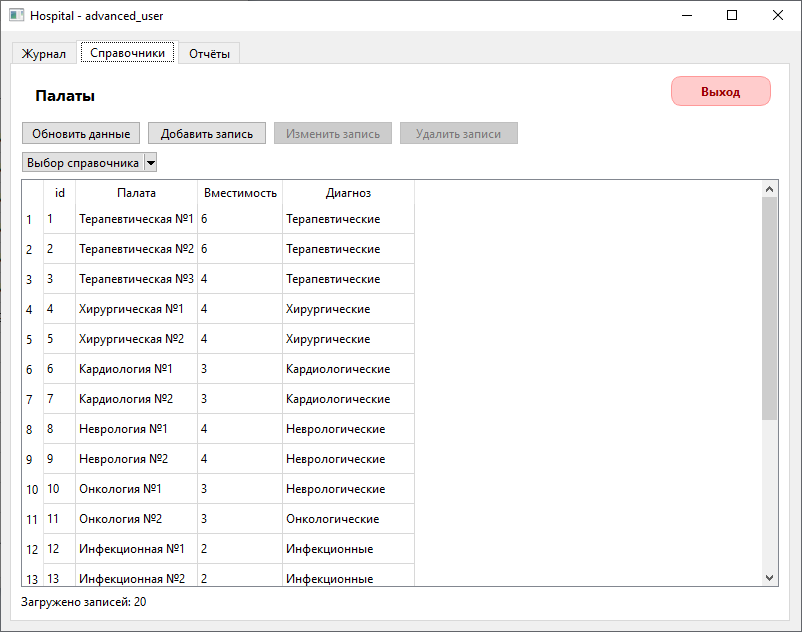
\includegraphics[width=0.75\textwidth]{images/directories_widget_01.png}
			\caption[]{Таблица палат для пользователя advanced\_user}
		\end{figure}
		\begin{figure}[H]
			\centering
			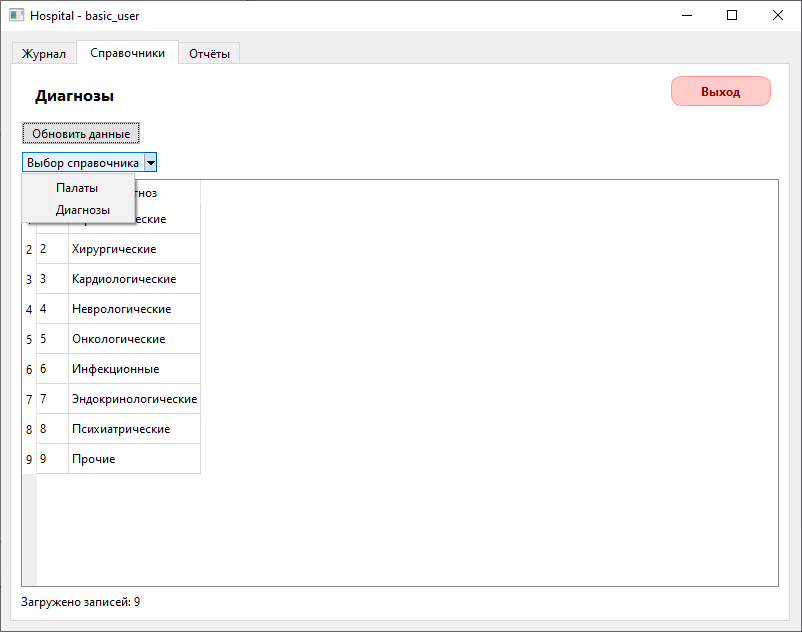
\includegraphics[width=0.75\textwidth]{images/directories_widget_1.png}
			\caption[]{Выбор справочника}
		\end{figure}
		Для палат выбор вместимости осуществляется с помощью spinbox, значения в котором ограничены диапазоном от 1 до 20.
		\begin{figure}[H]
			\centering
			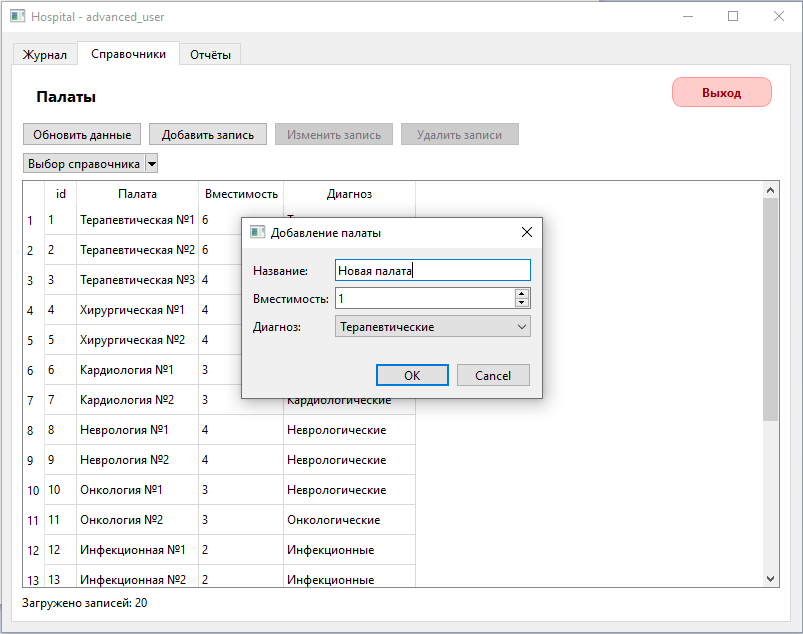
\includegraphics[width=0.75\textwidth]{images/directories_widget_2.png}
			\caption[]{Окно добавления/изменения палат}
		\end{figure}
		\begin{figure}[H]
			\centering
			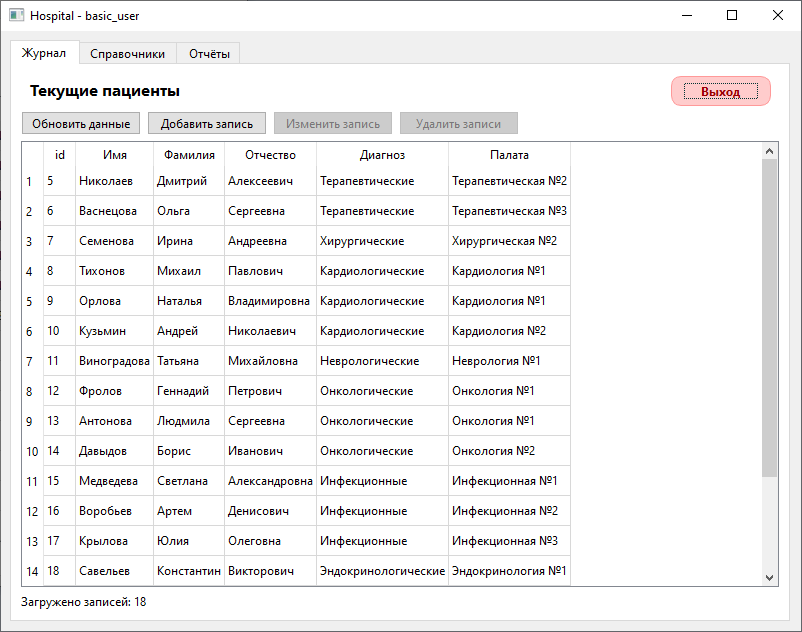
\includegraphics[width=0.75\textwidth]{images/main_widget_3.png}
			\caption[]{Результат удаления}
		\end{figure}
		\begin{figure}[H]
			\centering
			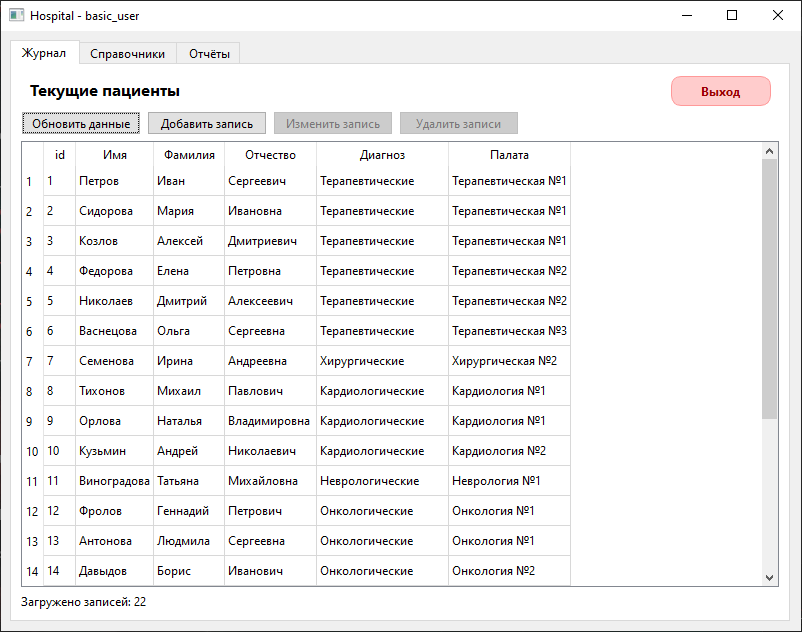
\includegraphics[width=0.75\textwidth]{images/main_widget_4.png}
			\caption[]{Неверный логин или пароль}
		\end{figure}
		\begin{figure}[H]
			\centering
			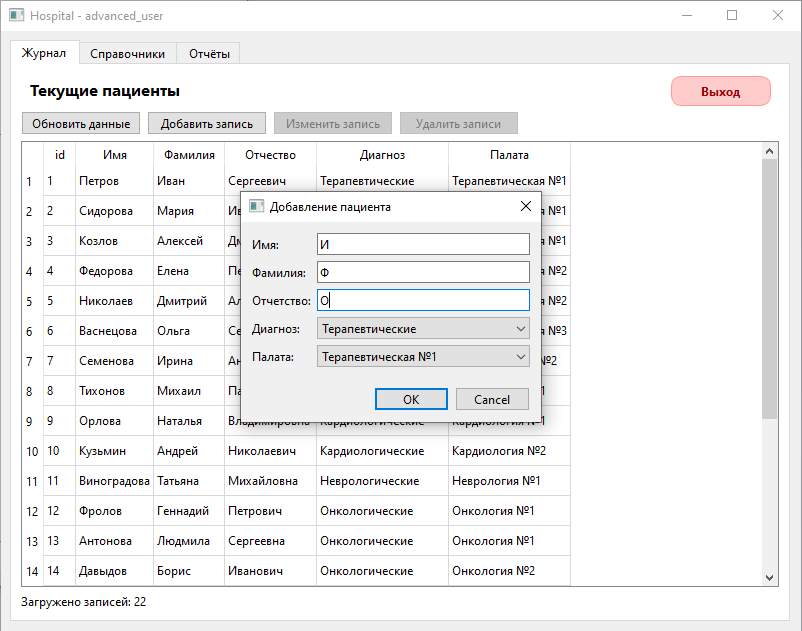
\includegraphics[width=0.75\textwidth]{images/main_widget_5.png}
			\caption[]{Окно добавления пациента}
		\end{figure}
		\begin{figure}[H]
			\centering
			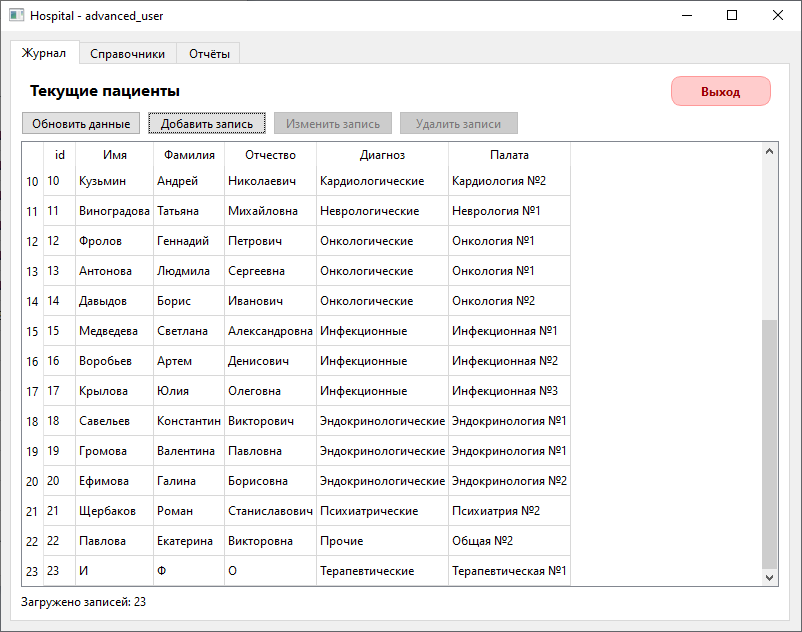
\includegraphics[width=0.75\textwidth]{images/main_widget_6.png}
			\caption[]{Результат добавления пациента}
		\end{figure}
		\begin{figure}[H]
			\centering
			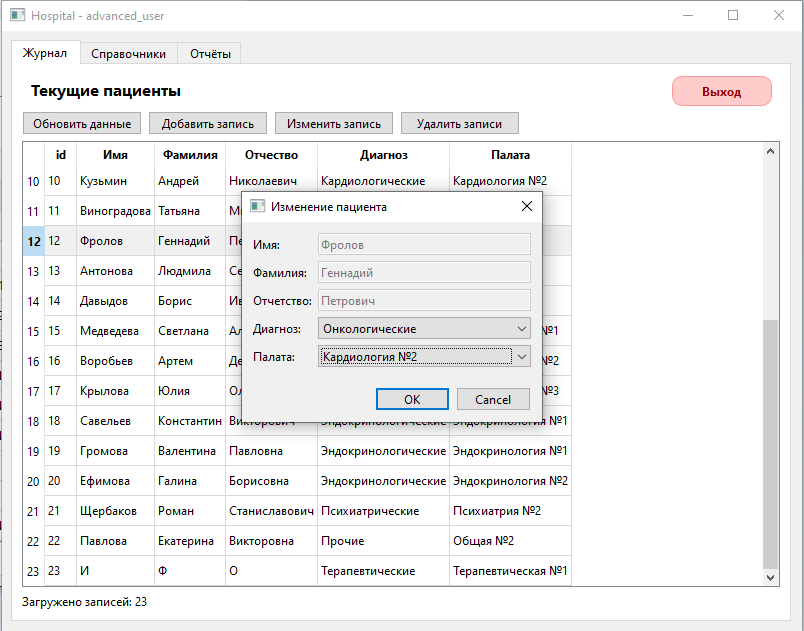
\includegraphics[width=0.75\textwidth]{images/main_widget_7.png}
			\caption[]{Окно изменения пациента}
		\end{figure}
		\begin{figure}[H]
			\centering
			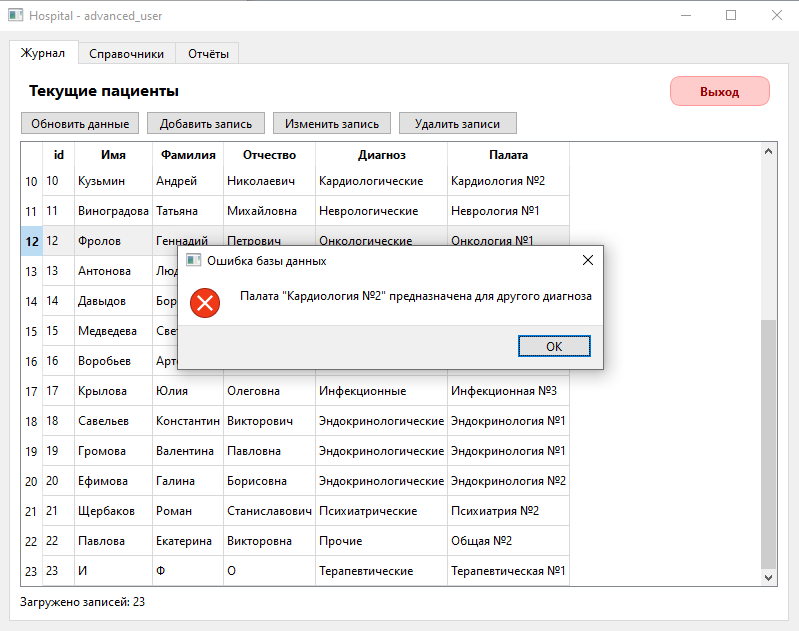
\includegraphics[width=0.75\textwidth]{images/main_widget_8.png}
			\caption[]{Ошибки при выборе некорректных данных}
		\end{figure}
	\subsubsection{Отчёты}
		\begin{figure}[H]
			\centering
			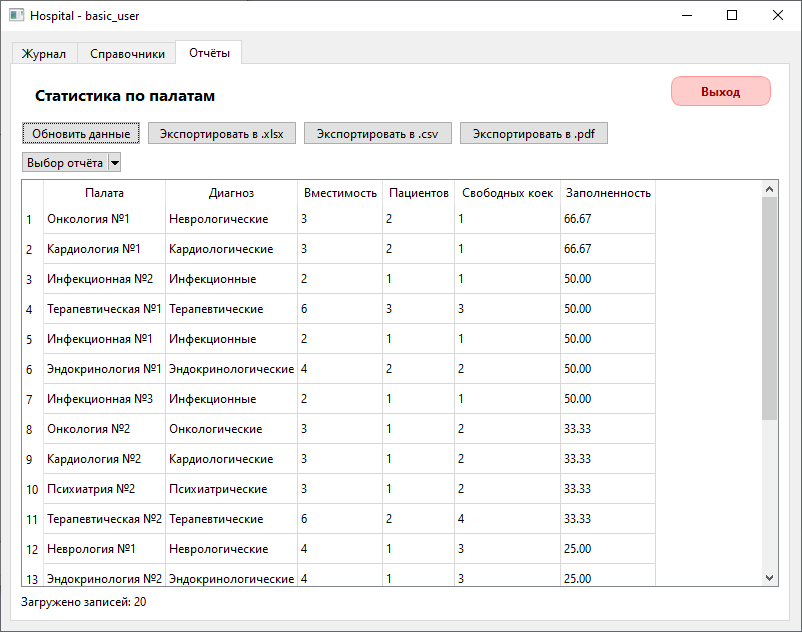
\includegraphics[width=0.75\textwidth]{images/reports_widget_0.png}
			\caption[]{Страницы отчётов}
		\end{figure}
		\begin{figure}[H]
			\centering
			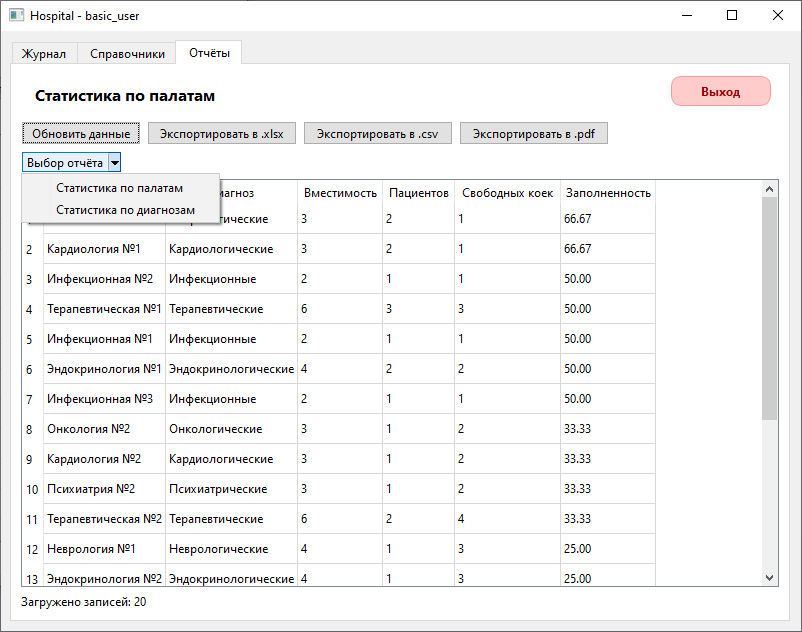
\includegraphics[width=0.75\textwidth]{images/reports_widget_1.png}
			\caption[]{Выбор отчёта}
		\end{figure}
		\begin{figure}[H]
			\centering
			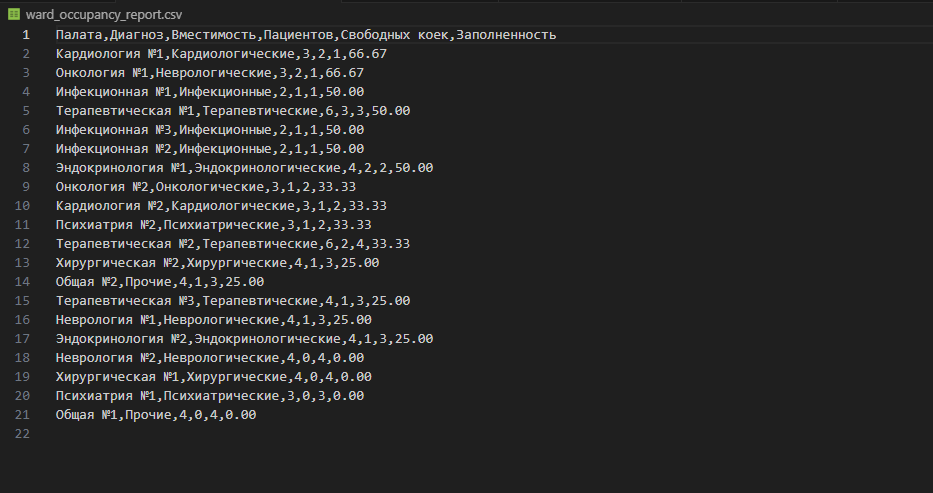
\includegraphics[width=0.75\textwidth]{images/csv_report.png}
			\caption[]{csv отчёт}
		\end{figure}
		\begin{figure}[H]
			\centering
			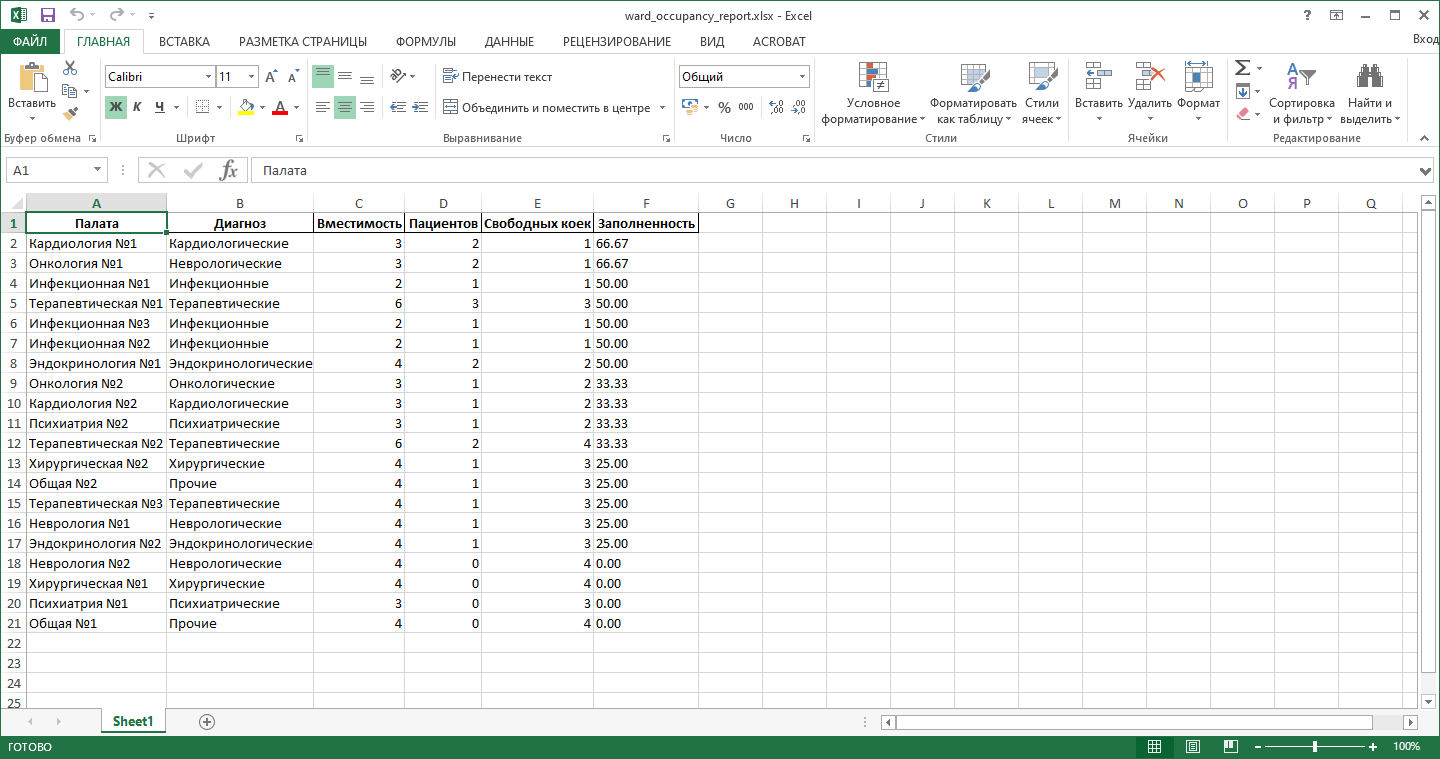
\includegraphics[width=0.75\textwidth]{images/xlsx_report.png}
			\caption[]{xlsx отчёт}
		\end{figure}
		\begin{figure}[H]
			\centering
			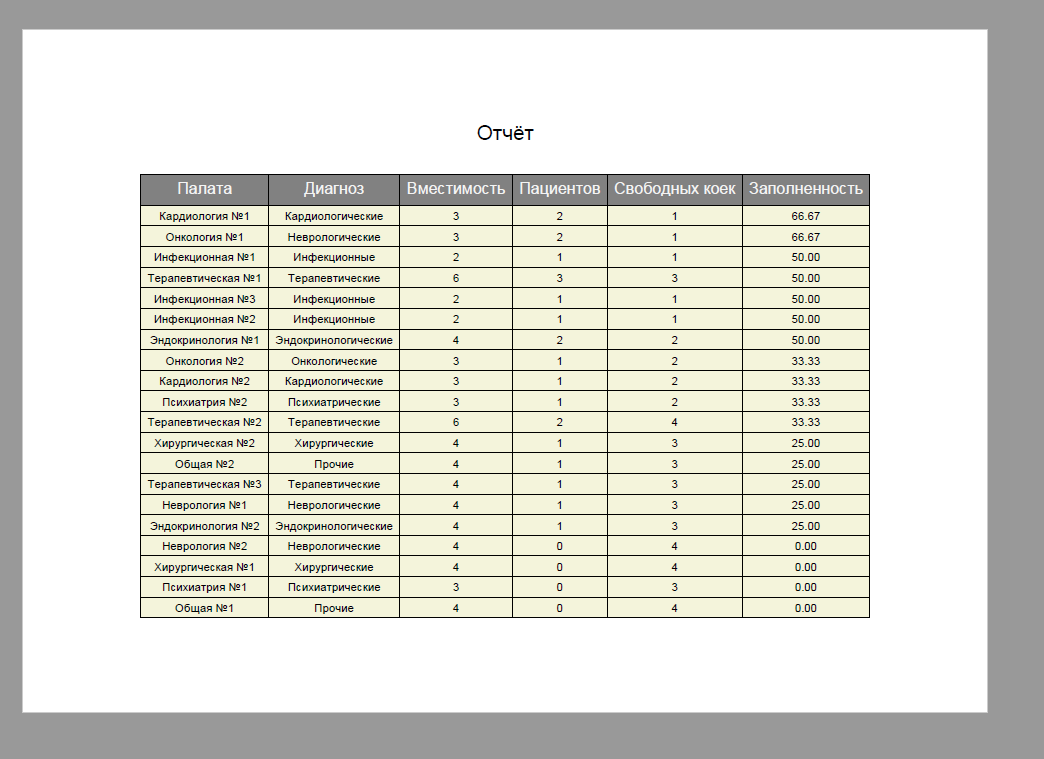
\includegraphics[width=0.75\textwidth]{images/pdf_report.png}
			\caption[]{pdf отчёт}
		\end{figure}
	\subsection{Выход}
	По нажатию на кнопку выхода открывается диалог с вариантами смены пользователя, который отправляет на начальный экран входа, или выход, который завершает выполнение программы.
	\begin{figure}[H]
		\centering
		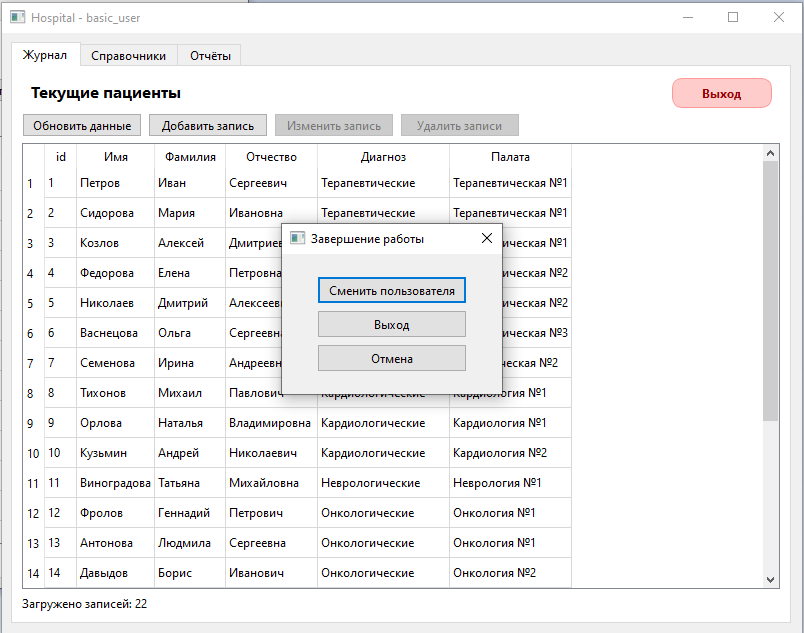
\includegraphics[width=0.75\textwidth]{images/exit_dialog.png}
		\caption[]{Диалог выхода и смены пользователя}
	\end{figure}
	
	\section{Вывод}
	\section{Список литературы}		
	
\end{document}